\documentclass[../../Main.tex]{subfiles}

\begin{document}
    \begin{figure}[hbt!]
        \centerline{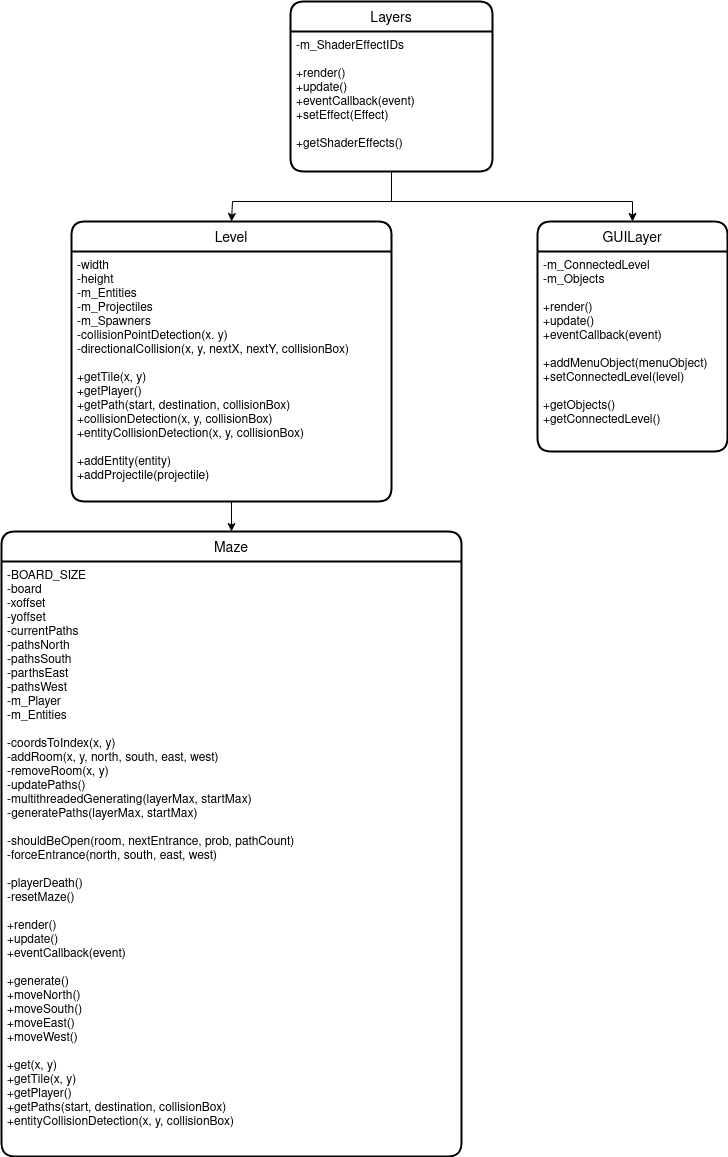
\includegraphics[scale=0.5]{img/Classes/Layers.png}}
        \caption{Layer subclasses}
        \label{fig}
    \end{figure}
    Layers
    \begin{center}
        Variables
        \begin{tabular}{ | m{0.45\textwidth} | m{0.45\textwidth} | }
            \hline
            \textbf{Variable Name} & \textbf{Description} \\
            \hline
            m\_ShaderEffectIDs & Stores the effects the layer needs when rendering \\
            \hline
        \end{tabular}
        Functions
        \begin{tabular}{ | m{0.15\textwidth} | m{0.35\textwidth}| m{0.4\textwidth} | }
            \hline
            \textbf{Function Name} & \textbf{Parameters} & \textbf{Description} \\
            \hline
            render & & Renders the layer \\
            \hline
            update & & Updates the layer \\
            \hline
            eventCallback & event that has happened & Allows the layer to interact with events \\
            \hline
            setEffect & effect & Sets an effect onto the layer (Will probably be an effect for the shader) \\
            \hline
            getShaderEffects & & Returns the shader effects for the layer \\
            \hline
        \end{tabular}
    \end{center}
    GUILayer
    \begin{center}
        Variables
        \begin{tabular}{ | m{0.45\textwidth} | m{0.45\textwidth} | }
            \hline
            \textbf{Variable Name} & \textbf{Description} \\
            \hline
            m\_ConnectedLevel & Stores the level it is connected to \\
            \hline
            m\_Objects & Stores the objects that are involved in the menu \\
            \hline
        \end{tabular}
        Functions
        \begin{tabular}{ | m{0.15\textwidth} | m{0.35\textwidth}| m{0.4\textwidth} | }
            \hline
            \textbf{Function Name} & \textbf{Parameters} & \textbf{Description} \\
            \hline
            addMenuObject & MenuObject to add & Adds a given menu object to the list of objects \\
            \hline
            setConnectedLevel & Level to connect to & Connects the layer to a given level (this does not need  to be set - only for menus interacting with the game) \\
            \hline
            getObjects & & Returns the list of objects that are involved in the menu \\
            \hline
            getConnectedLevel & & Returns the level the layer is connected to \\
            \hline
        \end{tabular}
    \end{center}
    Level
    \begin{center}
        Variables
        \begin{tabular}{ | m{0.45\textwidth} | m{0.45\textwidth} | }
            \hline
            \textbf{Variable Name} & \textbf{Description} \\
            \hline
            m\_Player & Stores the player on that level \\
            \hline
            width & Stores the width of the level (in terms of tiles)\\
            \hline
            height & Stores the height of the level (in terms of tiles)\\
            \hline
            m\_Entities & Stores a list of all the entities in the level \\
            \hline
            m\_Projectiles & Stores all the projectiles in the level \\
            \hline
            m\_Spawners & Stores all the current spawners in the level \\
            \hline
        \end{tabular}
        Functions
        \begin{tabular}{ | m{0.2\textwidth} | m{0.3\textwidth}| m{0.4\textwidth} | }
            \hline
            \textbf{Function Name} & \textbf{Parameters} & \textbf{Description} \\
            \hline
            collisionPointDetection & x and y of a point & Calculates whether a point is within a solid tile \\
            \hline
            directionalCollision & current x and y and the next x and y and the collision box of the object & Calculates whether an object is going to collide with any tile within the level \\
            \hline
            getTile & Tile x and y position in the level & Returns the tile at that point in time \\
            \hline
            getPlayer & & Returns the player \\
            \hline
            getPath & start position, end position and the collisionBox of the object & Returns a path of the shortest route between two points (using A* algorithm)\\
            \hline
            collisionDetection & x, y and collisionBox of an object & returns whether it has collided with anything \\
            \hline
            entityCollisionDetection & x, y and collisionBox of an object & returns whether it has collided with an entity in the level \\
            \hline
            addEntity & entity & Adds an entity to the level \\
            \hline
            addProjectile & projectile & Adds a projectile to the level \\
            \hline
            addSpawner & spawner & Adds a spawner to the level \\
            \hline
        \end{tabular}
    \end{center}
    Maze
    \begin{center}
        Variables
        \begin{tabular}{ | m{0.45\textwidth} | m{0.45\textwidth} | }
            \hline
            \textbf{Variable Name} & \textbf{Description} \\
            \hline
            BOARD\_SIZE & Static, constant variable that stores the width of the maze (in rooms) \\
            \hline
            board & Stores the list of rooms in the maze \\
            \hline
            xoffset & Stores the offset in the x direction for the top left corner of the maze \\
            \hline
            yoffset & Stores the offset in the y direction for the top left corner of the maze \\
            \hline
            currentPaths & Stores the current available paths the maze can generate in (used for generating the maze)\\
            \hline
            pathsNorth & Stores the paths that can be generated when the maze moves north \\
            \hline
            pathsSouth & Stores the paths that can be generated when the maze moves south \\
            \hline
            pathsEast & Stores the paths that can be generated when the maze moves east \\
            \hline
            pathsWest & Stores the paths that can be generated when the maze moves west \\
            \hline
        \end{tabular}
        Functions
        \begin{tabular}{ | m{0.2\textwidth} | m{0.3\textwidth}| m{0.4\textwidth} | }
            \hline
            \textbf{Function Name} & \textbf{Parameters} & \textbf{Description} \\
            \hline
            coordsToIndex & x and y position of a room & Converts a 2d coordinates for a room into an index of where it is in the board variable \\
            \hline
            addRoom & position and booleans for each entrance it could have & This adds a room at given coordinates, randomising what room it is and adding entities into it \\
            \hline
            removeRoom & x and y position of the room & This removes a room from the maze \\
            \hline
            updatePaths & & This updates the paths variables by resetting them and looking for new ones \\
            \hline
            multithreadedGenerating & The maximum layers for a boosted effect of generating and start maximum probability & This sets up everything needed to have the generating of the maze in another thread \\
            \hline
            generatePaths &  The maximum layers for a boosted effect of generating and start maximum probability & This is the function written in the prototype transferred for generating the maze using the currentPaths variable \\
            \hline
            shouldBeOpen & room, the next entrance, the probability of the entrance and count of how many entrances are already open & This returns an entrance state and chooses whether the entrance, should be open or closed (or it is closed but it could be opened)\\
            \hline
            forceEntrance & reference to the boolean values that store whether the entrance is going to be open or not & This will force an entrance, when the program believes there needs to be another entrance when generating \\
            \hline
            playerDeath & & This is the function that handles everything when the player dies \\
            \hline
            resetMaze & & This deals with resetting the whole maze \\
            \hline
            generate & & This is the function to call to generate a new maze \\
            \hline
            moveNorth & & This handles the maze moving to the north (and generates new rooms)\\
            \hline
            moveSouth & & This handles the maze moving to the south (and generates new rooms)\\
            \hline
            moveEast & & This handles the maze moving to the east (and generates new rooms) \\
            \hline
            moveWest & & This handles the maze moving to the west (and generates new rooms)\\
            \hline
            get & x and y pos of a room & This returns a room at the given coordinates \\
            \hline
        \end{tabular}
    \end{center}
\end{document}